% Created by tikzDevice version 0.12.3.1 on 2022-05-10 12:46:44
% !TEX encoding = UTF-8 Unicode
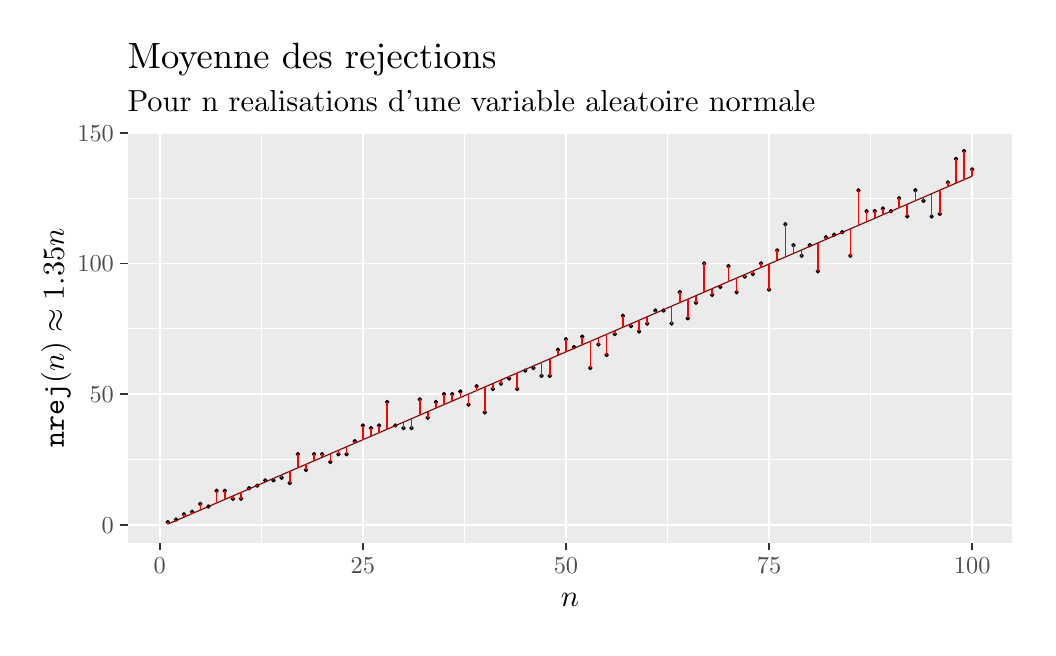
\begin{tikzpicture}[x=1pt,y=1pt]
\definecolor{fillColor}{RGB}{255,255,255}
\path[use as bounding box,fill=fillColor,fill opacity=0.00] (0,0) rectangle (361.35,216.81);
\begin{scope}
\path[clip] (  0.00,  0.00) rectangle (361.35,216.81);
\definecolor{drawColor}{RGB}{255,255,255}
\definecolor{fillColor}{RGB}{255,255,255}

\path[draw=drawColor,line width= 0.6pt,line join=round,line cap=round,fill=fillColor] (  0.00,  0.00) rectangle (361.35,216.81);
\end{scope}
\begin{scope}
\path[clip] ( 36.11, 30.69) rectangle (355.85,178.94);
\definecolor{fillColor}{gray}{0.92}

\path[fill=fillColor] ( 36.11, 30.69) rectangle (355.85,178.94);
\definecolor{drawColor}{RGB}{255,255,255}

\path[draw=drawColor,line width= 0.3pt,line join=round] ( 36.11, 60.78) --
	(355.85, 60.78);

\path[draw=drawColor,line width= 0.3pt,line join=round] ( 36.11,107.99) --
	(355.85,107.99);

\path[draw=drawColor,line width= 0.3pt,line join=round] ( 36.11,155.20) --
	(355.85,155.20);

\path[draw=drawColor,line width= 0.3pt,line join=round] ( 84.41, 30.69) --
	( 84.41,178.94);

\path[draw=drawColor,line width= 0.3pt,line join=round] (157.81, 30.69) --
	(157.81,178.94);

\path[draw=drawColor,line width= 0.3pt,line join=round] (231.21, 30.69) --
	(231.21,178.94);

\path[draw=drawColor,line width= 0.3pt,line join=round] (304.62, 30.69) --
	(304.62,178.94);

\path[draw=drawColor,line width= 0.6pt,line join=round] ( 36.11, 37.17) --
	(355.85, 37.17);

\path[draw=drawColor,line width= 0.6pt,line join=round] ( 36.11, 84.38) --
	(355.85, 84.38);

\path[draw=drawColor,line width= 0.6pt,line join=round] ( 36.11,131.60) --
	(355.85,131.60);

\path[draw=drawColor,line width= 0.6pt,line join=round] ( 36.11,178.81) --
	(355.85,178.81);

\path[draw=drawColor,line width= 0.6pt,line join=round] ( 47.71, 30.69) --
	( 47.71,178.94);

\path[draw=drawColor,line width= 0.6pt,line join=round] (121.11, 30.69) --
	(121.11,178.94);

\path[draw=drawColor,line width= 0.6pt,line join=round] (194.51, 30.69) --
	(194.51,178.94);

\path[draw=drawColor,line width= 0.6pt,line join=round] (267.91, 30.69) --
	(267.91,178.94);

\path[draw=drawColor,line width= 0.6pt,line join=round] (341.32, 30.69) --
	(341.32,178.94);
\definecolor{drawColor}{RGB}{0,0,0}
\definecolor{fillColor}{RGB}{0,0,0}

\path[draw=drawColor,line width= 0.4pt,line join=round,line cap=round,fill=fillColor] ( 50.64, 38.12) circle (  0.62);

\path[draw=drawColor,line width= 0.4pt,line join=round,line cap=round,fill=fillColor] ( 53.58, 39.06) circle (  0.62);

\path[draw=drawColor,line width= 0.4pt,line join=round,line cap=round,fill=fillColor] ( 56.52, 40.95) circle (  0.62);

\path[draw=drawColor,line width= 0.4pt,line join=round,line cap=round,fill=fillColor] ( 59.45, 41.89) circle (  0.62);

\path[draw=drawColor,line width= 0.4pt,line join=round,line cap=round,fill=fillColor] ( 62.39, 44.72) circle (  0.62);

\path[draw=drawColor,line width= 0.4pt,line join=round,line cap=round,fill=fillColor] ( 65.33, 43.78) circle (  0.62);

\path[draw=drawColor,line width= 0.4pt,line join=round,line cap=round,fill=fillColor] ( 68.26, 49.45) circle (  0.62);

\path[draw=drawColor,line width= 0.4pt,line join=round,line cap=round,fill=fillColor] ( 71.20, 49.45) circle (  0.62);

\path[draw=drawColor,line width= 0.4pt,line join=round,line cap=round,fill=fillColor] ( 74.13, 46.61) circle (  0.62);

\path[draw=drawColor,line width= 0.4pt,line join=round,line cap=round,fill=fillColor] ( 77.07, 46.61) circle (  0.62);

\path[draw=drawColor,line width= 0.4pt,line join=round,line cap=round,fill=fillColor] ( 80.01, 50.39) circle (  0.62);

\path[draw=drawColor,line width= 0.4pt,line join=round,line cap=round,fill=fillColor] ( 82.94, 51.33) circle (  0.62);

\path[draw=drawColor,line width= 0.4pt,line join=round,line cap=round,fill=fillColor] ( 85.88, 53.22) circle (  0.62);

\path[draw=drawColor,line width= 0.4pt,line join=round,line cap=round,fill=fillColor] ( 88.81, 53.22) circle (  0.62);

\path[draw=drawColor,line width= 0.4pt,line join=round,line cap=round,fill=fillColor] ( 91.75, 54.17) circle (  0.62);

\path[draw=drawColor,line width= 0.4pt,line join=round,line cap=round,fill=fillColor] ( 94.69, 52.28) circle (  0.62);

\path[draw=drawColor,line width= 0.4pt,line join=round,line cap=round,fill=fillColor] ( 97.62, 62.67) circle (  0.62);

\path[draw=drawColor,line width= 0.4pt,line join=round,line cap=round,fill=fillColor] (100.56, 57.00) circle (  0.62);

\path[draw=drawColor,line width= 0.4pt,line join=round,line cap=round,fill=fillColor] (103.49, 62.67) circle (  0.62);

\path[draw=drawColor,line width= 0.4pt,line join=round,line cap=round,fill=fillColor] (106.43, 62.67) circle (  0.62);

\path[draw=drawColor,line width= 0.4pt,line join=round,line cap=round,fill=fillColor] (109.37, 59.83) circle (  0.62);

\path[draw=drawColor,line width= 0.4pt,line join=round,line cap=round,fill=fillColor] (112.30, 62.67) circle (  0.62);

\path[draw=drawColor,line width= 0.4pt,line join=round,line cap=round,fill=fillColor] (115.24, 62.67) circle (  0.62);

\path[draw=drawColor,line width= 0.4pt,line join=round,line cap=round,fill=fillColor] (118.17, 67.39) circle (  0.62);

\path[draw=drawColor,line width= 0.4pt,line join=round,line cap=round,fill=fillColor] (121.11, 73.05) circle (  0.62);

\path[draw=drawColor,line width= 0.4pt,line join=round,line cap=round,fill=fillColor] (124.05, 72.11) circle (  0.62);

\path[draw=drawColor,line width= 0.4pt,line join=round,line cap=round,fill=fillColor] (126.98, 73.05) circle (  0.62);

\path[draw=drawColor,line width= 0.4pt,line join=round,line cap=round,fill=fillColor] (129.92, 81.55) circle (  0.62);

\path[draw=drawColor,line width= 0.4pt,line join=round,line cap=round,fill=fillColor] (132.85, 73.05) circle (  0.62);

\path[draw=drawColor,line width= 0.4pt,line join=round,line cap=round,fill=fillColor] (135.79, 72.11) circle (  0.62);

\path[draw=drawColor,line width= 0.4pt,line join=round,line cap=round,fill=fillColor] (138.73, 72.11) circle (  0.62);

\path[draw=drawColor,line width= 0.4pt,line join=round,line cap=round,fill=fillColor] (141.66, 82.50) circle (  0.62);

\path[draw=drawColor,line width= 0.4pt,line join=round,line cap=round,fill=fillColor] (144.60, 75.89) circle (  0.62);

\path[draw=drawColor,line width= 0.4pt,line join=round,line cap=round,fill=fillColor] (147.54, 81.55) circle (  0.62);

\path[draw=drawColor,line width= 0.4pt,line join=round,line cap=round,fill=fillColor] (150.47, 84.38) circle (  0.62);

\path[draw=drawColor,line width= 0.4pt,line join=round,line cap=round,fill=fillColor] (153.41, 84.38) circle (  0.62);

\path[draw=drawColor,line width= 0.4pt,line join=round,line cap=round,fill=fillColor] (156.34, 85.33) circle (  0.62);

\path[draw=drawColor,line width= 0.4pt,line join=round,line cap=round,fill=fillColor] (159.28, 80.61) circle (  0.62);

\path[draw=drawColor,line width= 0.4pt,line join=round,line cap=round,fill=fillColor] (162.22, 87.22) circle (  0.62);

\path[draw=drawColor,line width= 0.4pt,line join=round,line cap=round,fill=fillColor] (165.15, 77.77) circle (  0.62);

\path[draw=drawColor,line width= 0.4pt,line join=round,line cap=round,fill=fillColor] (168.09, 86.27) circle (  0.62);

\path[draw=drawColor,line width= 0.4pt,line join=round,line cap=round,fill=fillColor] (171.02, 88.16) circle (  0.62);

\path[draw=drawColor,line width= 0.4pt,line join=round,line cap=round,fill=fillColor] (173.96, 90.05) circle (  0.62);

\path[draw=drawColor,line width= 0.4pt,line join=round,line cap=round,fill=fillColor] (176.90, 86.27) circle (  0.62);

\path[draw=drawColor,line width= 0.4pt,line join=round,line cap=round,fill=fillColor] (179.83, 92.88) circle (  0.62);

\path[draw=drawColor,line width= 0.4pt,line join=round,line cap=round,fill=fillColor] (182.77, 93.83) circle (  0.62);

\path[draw=drawColor,line width= 0.4pt,line join=round,line cap=round,fill=fillColor] (185.70, 90.99) circle (  0.62);

\path[draw=drawColor,line width= 0.4pt,line join=round,line cap=round,fill=fillColor] (188.64, 90.99) circle (  0.62);

\path[draw=drawColor,line width= 0.4pt,line join=round,line cap=round,fill=fillColor] (191.58,100.44) circle (  0.62);

\path[draw=drawColor,line width= 0.4pt,line join=round,line cap=round,fill=fillColor] (194.51,104.21) circle (  0.62);

\path[draw=drawColor,line width= 0.4pt,line join=round,line cap=round,fill=fillColor] (197.45,101.38) circle (  0.62);

\path[draw=drawColor,line width= 0.4pt,line join=round,line cap=round,fill=fillColor] (200.38,105.16) circle (  0.62);

\path[draw=drawColor,line width= 0.4pt,line join=round,line cap=round,fill=fillColor] (203.32, 93.83) circle (  0.62);

\path[draw=drawColor,line width= 0.4pt,line join=round,line cap=round,fill=fillColor] (206.26,102.32) circle (  0.62);

\path[draw=drawColor,line width= 0.4pt,line join=round,line cap=round,fill=fillColor] (209.19, 98.55) circle (  0.62);

\path[draw=drawColor,line width= 0.4pt,line join=round,line cap=round,fill=fillColor] (212.13,106.10) circle (  0.62);

\path[draw=drawColor,line width= 0.4pt,line join=round,line cap=round,fill=fillColor] (215.07,112.71) circle (  0.62);

\path[draw=drawColor,line width= 0.4pt,line join=round,line cap=round,fill=fillColor] (218.00,108.93) circle (  0.62);

\path[draw=drawColor,line width= 0.4pt,line join=round,line cap=round,fill=fillColor] (220.94,107.05) circle (  0.62);

\path[draw=drawColor,line width= 0.4pt,line join=round,line cap=round,fill=fillColor] (223.87,109.88) circle (  0.62);

\path[draw=drawColor,line width= 0.4pt,line join=round,line cap=round,fill=fillColor] (226.81,114.60) circle (  0.62);

\path[draw=drawColor,line width= 0.4pt,line join=round,line cap=round,fill=fillColor] (229.75,114.60) circle (  0.62);

\path[draw=drawColor,line width= 0.4pt,line join=round,line cap=round,fill=fillColor] (232.68,109.88) circle (  0.62);

\path[draw=drawColor,line width= 0.4pt,line join=round,line cap=round,fill=fillColor] (235.62,121.21) circle (  0.62);

\path[draw=drawColor,line width= 0.4pt,line join=round,line cap=round,fill=fillColor] (238.55,111.77) circle (  0.62);

\path[draw=drawColor,line width= 0.4pt,line join=round,line cap=round,fill=fillColor] (241.49,117.43) circle (  0.62);

\path[draw=drawColor,line width= 0.4pt,line join=round,line cap=round,fill=fillColor] (244.43,131.60) circle (  0.62);

\path[draw=drawColor,line width= 0.4pt,line join=round,line cap=round,fill=fillColor] (247.36,120.27) circle (  0.62);

\path[draw=drawColor,line width= 0.4pt,line join=round,line cap=round,fill=fillColor] (250.30,123.10) circle (  0.62);

\path[draw=drawColor,line width= 0.4pt,line join=round,line cap=round,fill=fillColor] (253.23,130.65) circle (  0.62);

\path[draw=drawColor,line width= 0.4pt,line join=round,line cap=round,fill=fillColor] (256.17,121.21) circle (  0.62);

\path[draw=drawColor,line width= 0.4pt,line join=round,line cap=round,fill=fillColor] (259.11,126.88) circle (  0.62);

\path[draw=drawColor,line width= 0.4pt,line join=round,line cap=round,fill=fillColor] (262.04,127.82) circle (  0.62);

\path[draw=drawColor,line width= 0.4pt,line join=round,line cap=round,fill=fillColor] (264.98,131.60) circle (  0.62);

\path[draw=drawColor,line width= 0.4pt,line join=round,line cap=round,fill=fillColor] (267.91,122.15) circle (  0.62);

\path[draw=drawColor,line width= 0.4pt,line join=round,line cap=round,fill=fillColor] (270.85,136.32) circle (  0.62);

\path[draw=drawColor,line width= 0.4pt,line join=round,line cap=round,fill=fillColor] (273.79,145.76) circle (  0.62);

\path[draw=drawColor,line width= 0.4pt,line join=round,line cap=round,fill=fillColor] (276.72,138.21) circle (  0.62);

\path[draw=drawColor,line width= 0.4pt,line join=round,line cap=round,fill=fillColor] (279.66,134.43) circle (  0.62);

\path[draw=drawColor,line width= 0.4pt,line join=round,line cap=round,fill=fillColor] (282.59,138.21) circle (  0.62);

\path[draw=drawColor,line width= 0.4pt,line join=round,line cap=round,fill=fillColor] (285.53,128.76) circle (  0.62);

\path[draw=drawColor,line width= 0.4pt,line join=round,line cap=round,fill=fillColor] (288.47,141.04) circle (  0.62);

\path[draw=drawColor,line width= 0.4pt,line join=round,line cap=round,fill=fillColor] (291.40,141.98) circle (  0.62);

\path[draw=drawColor,line width= 0.4pt,line join=round,line cap=round,fill=fillColor] (294.34,142.93) circle (  0.62);

\path[draw=drawColor,line width= 0.4pt,line join=round,line cap=round,fill=fillColor] (297.28,134.43) circle (  0.62);

\path[draw=drawColor,line width= 0.4pt,line join=round,line cap=round,fill=fillColor] (300.21,158.04) circle (  0.62);

\path[draw=drawColor,line width= 0.4pt,line join=round,line cap=round,fill=fillColor] (303.15,150.48) circle (  0.62);

\path[draw=drawColor,line width= 0.4pt,line join=round,line cap=round,fill=fillColor] (306.08,150.48) circle (  0.62);

\path[draw=drawColor,line width= 0.4pt,line join=round,line cap=round,fill=fillColor] (309.02,151.43) circle (  0.62);

\path[draw=drawColor,line width= 0.4pt,line join=round,line cap=round,fill=fillColor] (311.96,150.48) circle (  0.62);

\path[draw=drawColor,line width= 0.4pt,line join=round,line cap=round,fill=fillColor] (314.89,155.20) circle (  0.62);

\path[draw=drawColor,line width= 0.4pt,line join=round,line cap=round,fill=fillColor] (317.83,148.59) circle (  0.62);

\path[draw=drawColor,line width= 0.4pt,line join=round,line cap=round,fill=fillColor] (320.76,158.04) circle (  0.62);

\path[draw=drawColor,line width= 0.4pt,line join=round,line cap=round,fill=fillColor] (323.70,154.26) circle (  0.62);

\path[draw=drawColor,line width= 0.4pt,line join=round,line cap=round,fill=fillColor] (326.64,148.59) circle (  0.62);

\path[draw=drawColor,line width= 0.4pt,line join=round,line cap=round,fill=fillColor] (329.57,149.54) circle (  0.62);

\path[draw=drawColor,line width= 0.4pt,line join=round,line cap=round,fill=fillColor] (332.51,160.87) circle (  0.62);

\path[draw=drawColor,line width= 0.4pt,line join=round,line cap=round,fill=fillColor] (335.44,169.37) circle (  0.62);

\path[draw=drawColor,line width= 0.4pt,line join=round,line cap=round,fill=fillColor] (338.38,172.20) circle (  0.62);

\path[draw=drawColor,line width= 0.4pt,line join=round,line cap=round,fill=fillColor] (341.32,165.59) circle (  0.62);

\path[draw=drawColor,line width= 0.3pt,line join=round] ( 50.64, 37.42) --
	( 53.58, 38.69) --
	( 56.52, 39.96) --
	( 59.45, 41.23) --
	( 62.39, 42.50) --
	( 65.33, 43.78) --
	( 68.26, 45.05) --
	( 71.20, 46.32) --
	( 74.13, 47.59) --
	( 77.07, 48.86) --
	( 80.01, 50.13) --
	( 82.94, 51.40) --
	( 85.88, 52.67) --
	( 88.81, 53.94) --
	( 91.75, 55.21) --
	( 94.69, 56.48) --
	( 97.62, 57.75) --
	(100.56, 59.02) --
	(103.49, 60.29) --
	(106.43, 61.56) --
	(109.37, 62.83) --
	(112.30, 64.10) --
	(115.24, 65.37) --
	(118.17, 66.64) --
	(121.11, 67.91) --
	(124.05, 69.18) --
	(126.98, 70.45) --
	(129.92, 71.72) --
	(132.85, 72.99) --
	(135.79, 74.26) --
	(138.73, 75.53) --
	(141.66, 76.80) --
	(144.60, 78.07) --
	(147.54, 79.34) --
	(150.47, 80.61) --
	(153.41, 81.88) --
	(156.34, 83.15) --
	(159.28, 84.42) --
	(162.22, 85.69) --
	(165.15, 86.96) --
	(168.09, 88.23) --
	(171.02, 89.50) --
	(173.96, 90.77) --
	(176.90, 92.04) --
	(179.83, 93.31) --
	(182.77, 94.58) --
	(185.70, 95.85) --
	(188.64, 97.12) --
	(191.58, 98.39) --
	(194.51, 99.66) --
	(197.45,100.93) --
	(200.38,102.20) --
	(203.32,103.47) --
	(206.26,104.74) --
	(209.19,106.01) --
	(212.13,107.28) --
	(215.07,108.55) --
	(218.00,109.82) --
	(220.94,111.09) --
	(223.87,112.36) --
	(226.81,113.63) --
	(229.75,114.90) --
	(232.68,116.17) --
	(235.62,117.44) --
	(238.55,118.71) --
	(241.49,119.98) --
	(244.43,121.25) --
	(247.36,122.52) --
	(250.30,123.79) --
	(253.23,125.06) --
	(256.17,126.33) --
	(259.11,127.60) --
	(262.04,128.87) --
	(264.98,130.14) --
	(267.91,131.41) --
	(270.85,132.68) --
	(273.79,133.95) --
	(276.72,135.22) --
	(279.66,136.49) --
	(282.59,137.76) --
	(285.53,139.03) --
	(288.47,140.30) --
	(291.40,141.57) --
	(294.34,142.84) --
	(297.28,144.11) --
	(300.21,145.38) --
	(303.15,146.65) --
	(306.08,147.92) --
	(309.02,149.19) --
	(311.96,150.46) --
	(314.89,151.73) --
	(317.83,153.00) --
	(320.76,154.27) --
	(323.70,155.54) --
	(326.64,156.81) --
	(329.57,158.08) --
	(332.51,159.35) --
	(335.44,160.62) --
	(338.38,161.89) --
	(341.32,163.16);
\definecolor{drawColor}{RGB}{255,0,0}

\path[draw=drawColor,draw opacity=0.30,line width= 0.6pt,line join=round] ( 50.64, 37.42) --
	( 53.58, 38.69) --
	( 56.52, 39.96) --
	( 59.45, 41.23) --
	( 62.39, 42.50) --
	( 65.33, 43.78) --
	( 68.26, 45.05) --
	( 71.20, 46.32) --
	( 74.13, 47.59) --
	( 77.07, 48.86) --
	( 80.01, 50.13) --
	( 82.94, 51.40) --
	( 85.88, 52.67) --
	( 88.81, 53.94) --
	( 91.75, 55.21) --
	( 94.69, 56.48) --
	( 97.62, 57.75) --
	(100.56, 59.02) --
	(103.49, 60.29) --
	(106.43, 61.56) --
	(109.37, 62.83) --
	(112.30, 64.10) --
	(115.24, 65.37) --
	(118.17, 66.64) --
	(121.11, 67.91) --
	(124.05, 69.18) --
	(126.98, 70.45) --
	(129.92, 71.72) --
	(132.85, 72.99) --
	(135.79, 74.26) --
	(138.73, 75.53) --
	(141.66, 76.80) --
	(144.60, 78.07) --
	(147.54, 79.34) --
	(150.47, 80.61) --
	(153.41, 81.88) --
	(156.34, 83.15) --
	(159.28, 84.42) --
	(162.22, 85.69) --
	(165.15, 86.96) --
	(168.09, 88.23) --
	(171.02, 89.50) --
	(173.96, 90.77) --
	(176.90, 92.04) --
	(179.83, 93.31) --
	(182.77, 94.58) --
	(185.70, 95.85) --
	(188.64, 97.12) --
	(191.58, 98.39) --
	(194.51, 99.66) --
	(197.45,100.93) --
	(200.38,102.20) --
	(203.32,103.47) --
	(206.26,104.74) --
	(209.19,106.01) --
	(212.13,107.28) --
	(215.07,108.55) --
	(218.00,109.82) --
	(220.94,111.09) --
	(223.87,112.36) --
	(226.81,113.63) --
	(229.75,114.90) --
	(232.68,116.17) --
	(235.62,117.44) --
	(238.55,118.71) --
	(241.49,119.98) --
	(244.43,121.25) --
	(247.36,122.52) --
	(250.30,123.79) --
	(253.23,125.06) --
	(256.17,126.33) --
	(259.11,127.60) --
	(262.04,128.87) --
	(264.98,130.14) --
	(267.91,131.41) --
	(270.85,132.68) --
	(273.79,133.95) --
	(276.72,135.22) --
	(279.66,136.49) --
	(282.59,137.76) --
	(285.53,139.03) --
	(288.47,140.30) --
	(291.40,141.57) --
	(294.34,142.84) --
	(297.28,144.11) --
	(300.21,145.38) --
	(303.15,146.65) --
	(306.08,147.92) --
	(309.02,149.19) --
	(311.96,150.46) --
	(314.89,151.73) --
	(317.83,153.00) --
	(320.76,154.27) --
	(323.70,155.54) --
	(326.64,156.81) --
	(329.57,158.08) --
	(332.51,159.35) --
	(335.44,160.62) --
	(338.38,161.89) --
	(341.32,163.16);
\definecolor{drawColor}{RGB}{255,0,0}

\path[draw=drawColor,line width= 0.6pt,line join=round] ( 50.64, 37.42) -- ( 50.64, 38.12);

\path[draw=drawColor,line width= 0.6pt,line join=round] ( 53.58, 38.69) -- ( 53.58, 39.06);

\path[draw=drawColor,line width= 0.6pt,line join=round] ( 56.52, 39.96) -- ( 56.52, 40.95);

\path[draw=drawColor,line width= 0.6pt,line join=round] ( 59.45, 41.23) -- ( 59.45, 41.89);

\path[draw=drawColor,line width= 0.6pt,line join=round] ( 62.39, 42.50) -- ( 62.39, 44.72);

\path[draw=drawColor,line width= 0.6pt,line join=round] ( 65.33, 43.78) -- ( 65.33, 43.78);

\path[draw=drawColor,line width= 0.6pt,line join=round] ( 68.26, 45.05) -- ( 68.26, 49.45);

\path[draw=drawColor,line width= 0.6pt,line join=round] ( 71.20, 46.32) -- ( 71.20, 49.45);

\path[draw=drawColor,line width= 0.6pt,line join=round] ( 74.13, 47.59) -- ( 74.13, 46.61);

\path[draw=drawColor,line width= 0.6pt,line join=round] ( 77.07, 48.86) -- ( 77.07, 46.61);

\path[draw=drawColor,line width= 0.6pt,line join=round] ( 80.01, 50.13) -- ( 80.01, 50.39);

\path[draw=drawColor,line width= 0.6pt,line join=round] ( 82.94, 51.40) -- ( 82.94, 51.33);

\path[draw=drawColor,line width= 0.6pt,line join=round] ( 85.88, 52.67) -- ( 85.88, 53.22);

\path[draw=drawColor,line width= 0.6pt,line join=round] ( 88.81, 53.94) -- ( 88.81, 53.22);

\path[draw=drawColor,line width= 0.6pt,line join=round] ( 91.75, 55.21) -- ( 91.75, 54.17);

\path[draw=drawColor,line width= 0.6pt,line join=round] ( 94.69, 56.48) -- ( 94.69, 52.28);

\path[draw=drawColor,line width= 0.6pt,line join=round] ( 97.62, 57.75) -- ( 97.62, 62.67);

\path[draw=drawColor,line width= 0.6pt,line join=round] (100.56, 59.02) -- (100.56, 57.00);

\path[draw=drawColor,line width= 0.6pt,line join=round] (103.49, 60.29) -- (103.49, 62.67);

\path[draw=drawColor,line width= 0.6pt,line join=round] (106.43, 61.56) -- (106.43, 62.67);

\path[draw=drawColor,line width= 0.6pt,line join=round] (109.37, 62.83) -- (109.37, 59.83);

\path[draw=drawColor,line width= 0.6pt,line join=round] (112.30, 64.10) -- (112.30, 62.67);

\path[draw=drawColor,line width= 0.6pt,line join=round] (115.24, 65.37) -- (115.24, 62.67);

\path[draw=drawColor,line width= 0.6pt,line join=round] (118.17, 66.64) -- (118.17, 67.39);

\path[draw=drawColor,line width= 0.6pt,line join=round] (121.11, 67.91) -- (121.11, 73.05);

\path[draw=drawColor,line width= 0.6pt,line join=round] (124.05, 69.18) -- (124.05, 72.11);

\path[draw=drawColor,line width= 0.6pt,line join=round] (126.98, 70.45) -- (126.98, 73.05);

\path[draw=drawColor,line width= 0.6pt,line join=round] (129.92, 71.72) -- (129.92, 81.55);

\path[draw=drawColor,line width= 0.6pt,line join=round] (132.85, 72.99) -- (132.85, 73.05);

\path[draw=drawColor,line width= 0.6pt,line join=round] (135.79, 74.26) -- (135.79, 72.11);

\path[draw=drawColor,line width= 0.6pt,line join=round] (138.73, 75.53) -- (138.73, 72.11);

\path[draw=drawColor,line width= 0.6pt,line join=round] (141.66, 76.80) -- (141.66, 82.50);

\path[draw=drawColor,line width= 0.6pt,line join=round] (144.60, 78.07) -- (144.60, 75.89);

\path[draw=drawColor,line width= 0.6pt,line join=round] (147.54, 79.34) -- (147.54, 81.55);

\path[draw=drawColor,line width= 0.6pt,line join=round] (150.47, 80.61) -- (150.47, 84.38);

\path[draw=drawColor,line width= 0.6pt,line join=round] (153.41, 81.88) -- (153.41, 84.38);

\path[draw=drawColor,line width= 0.6pt,line join=round] (156.34, 83.15) -- (156.34, 85.33);

\path[draw=drawColor,line width= 0.6pt,line join=round] (159.28, 84.42) -- (159.28, 80.61);

\path[draw=drawColor,line width= 0.6pt,line join=round] (162.22, 85.69) -- (162.22, 87.22);

\path[draw=drawColor,line width= 0.6pt,line join=round] (165.15, 86.96) -- (165.15, 77.77);

\path[draw=drawColor,line width= 0.6pt,line join=round] (168.09, 88.23) -- (168.09, 86.27);

\path[draw=drawColor,line width= 0.6pt,line join=round] (171.02, 89.50) -- (171.02, 88.16);

\path[draw=drawColor,line width= 0.6pt,line join=round] (173.96, 90.77) -- (173.96, 90.05);

\path[draw=drawColor,line width= 0.6pt,line join=round] (176.90, 92.04) -- (176.90, 86.27);

\path[draw=drawColor,line width= 0.6pt,line join=round] (179.83, 93.31) -- (179.83, 92.88);

\path[draw=drawColor,line width= 0.6pt,line join=round] (182.77, 94.58) -- (182.77, 93.83);

\path[draw=drawColor,line width= 0.6pt,line join=round] (185.70, 95.85) -- (185.70, 90.99);

\path[draw=drawColor,line width= 0.6pt,line join=round] (188.64, 97.12) -- (188.64, 90.99);

\path[draw=drawColor,line width= 0.6pt,line join=round] (191.58, 98.39) -- (191.58,100.44);

\path[draw=drawColor,line width= 0.6pt,line join=round] (194.51, 99.66) -- (194.51,104.21);

\path[draw=drawColor,line width= 0.6pt,line join=round] (197.45,100.93) -- (197.45,101.38);

\path[draw=drawColor,line width= 0.6pt,line join=round] (200.38,102.20) -- (200.38,105.16);

\path[draw=drawColor,line width= 0.6pt,line join=round] (203.32,103.47) -- (203.32, 93.83);

\path[draw=drawColor,line width= 0.6pt,line join=round] (206.26,104.74) -- (206.26,102.32);

\path[draw=drawColor,line width= 0.6pt,line join=round] (209.19,106.01) -- (209.19, 98.55);

\path[draw=drawColor,line width= 0.6pt,line join=round] (212.13,107.28) -- (212.13,106.10);

\path[draw=drawColor,line width= 0.6pt,line join=round] (215.07,108.55) -- (215.07,112.71);

\path[draw=drawColor,line width= 0.6pt,line join=round] (218.00,109.82) -- (218.00,108.93);

\path[draw=drawColor,line width= 0.6pt,line join=round] (220.94,111.09) -- (220.94,107.05);

\path[draw=drawColor,line width= 0.6pt,line join=round] (223.87,112.36) -- (223.87,109.88);

\path[draw=drawColor,line width= 0.6pt,line join=round] (226.81,113.63) -- (226.81,114.60);

\path[draw=drawColor,line width= 0.6pt,line join=round] (229.75,114.90) -- (229.75,114.60);

\path[draw=drawColor,line width= 0.6pt,line join=round] (232.68,116.17) -- (232.68,109.88);

\path[draw=drawColor,line width= 0.6pt,line join=round] (235.62,117.44) -- (235.62,121.21);

\path[draw=drawColor,line width= 0.6pt,line join=round] (238.55,118.71) -- (238.55,111.77);

\path[draw=drawColor,line width= 0.6pt,line join=round] (241.49,119.98) -- (241.49,117.43);

\path[draw=drawColor,line width= 0.6pt,line join=round] (244.43,121.25) -- (244.43,131.60);

\path[draw=drawColor,line width= 0.6pt,line join=round] (247.36,122.52) -- (247.36,120.27);

\path[draw=drawColor,line width= 0.6pt,line join=round] (250.30,123.79) -- (250.30,123.10);

\path[draw=drawColor,line width= 0.6pt,line join=round] (253.23,125.06) -- (253.23,130.65);

\path[draw=drawColor,line width= 0.6pt,line join=round] (256.17,126.33) -- (256.17,121.21);

\path[draw=drawColor,line width= 0.6pt,line join=round] (259.11,127.60) -- (259.11,126.88);

\path[draw=drawColor,line width= 0.6pt,line join=round] (262.04,128.87) -- (262.04,127.82);

\path[draw=drawColor,line width= 0.6pt,line join=round] (264.98,130.14) -- (264.98,131.60);

\path[draw=drawColor,line width= 0.6pt,line join=round] (267.91,131.41) -- (267.91,122.15);

\path[draw=drawColor,line width= 0.6pt,line join=round] (270.85,132.68) -- (270.85,136.32);

\path[draw=drawColor,line width= 0.6pt,line join=round] (273.79,133.95) -- (273.79,145.76);

\path[draw=drawColor,line width= 0.6pt,line join=round] (276.72,135.22) -- (276.72,138.21);

\path[draw=drawColor,line width= 0.6pt,line join=round] (279.66,136.49) -- (279.66,134.43);

\path[draw=drawColor,line width= 0.6pt,line join=round] (282.59,137.76) -- (282.59,138.21);

\path[draw=drawColor,line width= 0.6pt,line join=round] (285.53,139.03) -- (285.53,128.76);

\path[draw=drawColor,line width= 0.6pt,line join=round] (288.47,140.30) -- (288.47,141.04);

\path[draw=drawColor,line width= 0.6pt,line join=round] (291.40,141.57) -- (291.40,141.98);

\path[draw=drawColor,line width= 0.6pt,line join=round] (294.34,142.84) -- (294.34,142.93);

\path[draw=drawColor,line width= 0.6pt,line join=round] (297.28,144.11) -- (297.28,134.43);

\path[draw=drawColor,line width= 0.6pt,line join=round] (300.21,145.38) -- (300.21,158.04);

\path[draw=drawColor,line width= 0.6pt,line join=round] (303.15,146.65) -- (303.15,150.48);

\path[draw=drawColor,line width= 0.6pt,line join=round] (306.08,147.92) -- (306.08,150.48);

\path[draw=drawColor,line width= 0.6pt,line join=round] (309.02,149.19) -- (309.02,151.43);

\path[draw=drawColor,line width= 0.6pt,line join=round] (311.96,150.46) -- (311.96,150.48);

\path[draw=drawColor,line width= 0.6pt,line join=round] (314.89,151.73) -- (314.89,155.20);

\path[draw=drawColor,line width= 0.6pt,line join=round] (317.83,153.00) -- (317.83,148.59);

\path[draw=drawColor,line width= 0.6pt,line join=round] (320.76,154.27) -- (320.76,158.04);

\path[draw=drawColor,line width= 0.6pt,line join=round] (323.70,155.54) -- (323.70,154.26);

\path[draw=drawColor,line width= 0.6pt,line join=round] (326.64,156.81) -- (326.64,148.59);

\path[draw=drawColor,line width= 0.6pt,line join=round] (329.57,158.08) -- (329.57,149.54);

\path[draw=drawColor,line width= 0.6pt,line join=round] (332.51,159.35) -- (332.51,160.87);

\path[draw=drawColor,line width= 0.6pt,line join=round] (335.44,160.62) -- (335.44,169.37);

\path[draw=drawColor,line width= 0.6pt,line join=round] (338.38,161.89) -- (338.38,172.20);

\path[draw=drawColor,line width= 0.6pt,line join=round] (341.32,163.16) -- (341.32,165.59);
\end{scope}
\begin{scope}
\path[clip] (  0.00,  0.00) rectangle (361.35,216.81);
\definecolor{drawColor}{gray}{0.30}

\node[text=drawColor,anchor=base east,inner sep=0pt, outer sep=0pt, scale=  0.88] at ( 31.16, 34.14) {0};

\node[text=drawColor,anchor=base east,inner sep=0pt, outer sep=0pt, scale=  0.88] at ( 31.16, 81.35) {50};

\node[text=drawColor,anchor=base east,inner sep=0pt, outer sep=0pt, scale=  0.88] at ( 31.16,128.57) {100};

\node[text=drawColor,anchor=base east,inner sep=0pt, outer sep=0pt, scale=  0.88] at ( 31.16,175.78) {150};
\end{scope}
\begin{scope}
\path[clip] (  0.00,  0.00) rectangle (361.35,216.81);
\definecolor{drawColor}{gray}{0.20}

\path[draw=drawColor,line width= 0.6pt,line join=round] ( 33.36, 37.17) --
	( 36.11, 37.17);

\path[draw=drawColor,line width= 0.6pt,line join=round] ( 33.36, 84.38) --
	( 36.11, 84.38);

\path[draw=drawColor,line width= 0.6pt,line join=round] ( 33.36,131.60) --
	( 36.11,131.60);

\path[draw=drawColor,line width= 0.6pt,line join=round] ( 33.36,178.81) --
	( 36.11,178.81);
\end{scope}
\begin{scope}
\path[clip] (  0.00,  0.00) rectangle (361.35,216.81);
\definecolor{drawColor}{gray}{0.20}

\path[draw=drawColor,line width= 0.6pt,line join=round] ( 47.71, 27.94) --
	( 47.71, 30.69);

\path[draw=drawColor,line width= 0.6pt,line join=round] (121.11, 27.94) --
	(121.11, 30.69);

\path[draw=drawColor,line width= 0.6pt,line join=round] (194.51, 27.94) --
	(194.51, 30.69);

\path[draw=drawColor,line width= 0.6pt,line join=round] (267.91, 27.94) --
	(267.91, 30.69);

\path[draw=drawColor,line width= 0.6pt,line join=round] (341.32, 27.94) --
	(341.32, 30.69);
\end{scope}
\begin{scope}
\path[clip] (  0.00,  0.00) rectangle (361.35,216.81);
\definecolor{drawColor}{gray}{0.30}

\node[text=drawColor,anchor=base,inner sep=0pt, outer sep=0pt, scale=  0.88] at ( 47.71, 19.68) {0};

\node[text=drawColor,anchor=base,inner sep=0pt, outer sep=0pt, scale=  0.88] at (121.11, 19.68) {25};

\node[text=drawColor,anchor=base,inner sep=0pt, outer sep=0pt, scale=  0.88] at (194.51, 19.68) {50};

\node[text=drawColor,anchor=base,inner sep=0pt, outer sep=0pt, scale=  0.88] at (267.91, 19.68) {75};

\node[text=drawColor,anchor=base,inner sep=0pt, outer sep=0pt, scale=  0.88] at (341.32, 19.68) {100};
\end{scope}
\begin{scope}
\path[clip] (  0.00,  0.00) rectangle (361.35,216.81);
\definecolor{drawColor}{RGB}{0,0,0}

\node[text=drawColor,anchor=base,inner sep=0pt, outer sep=0pt, scale=  1.10] at (195.98,  7.64) {$n$};
\end{scope}
\begin{scope}
\path[clip] (  0.00,  0.00) rectangle (361.35,216.81);
\definecolor{drawColor}{RGB}{0,0,0}

\node[text=drawColor,rotate= 90.00,anchor=base,inner sep=0pt, outer sep=0pt, scale=  1.10] at ( 13.08,104.81) {$\texttt{nrej}(n) \approx 1.35n$};
\end{scope}
\begin{scope}
\path[clip] (  0.00,  0.00) rectangle (361.35,216.81);
\definecolor{drawColor}{RGB}{0,0,0}

\node[text=drawColor,anchor=base west,inner sep=0pt, outer sep=0pt, scale=  1.10] at ( 36.11,186.58) {Pour n realisations d'une variable aleatoire normale};
\end{scope}
\begin{scope}
\path[clip] (  0.00,  0.00) rectangle (361.35,216.81);
\definecolor{drawColor}{RGB}{0,0,0}

\node[text=drawColor,anchor=base west,inner sep=0pt, outer sep=0pt, scale=  1.32] at ( 36.11,202.22) {Moyenne des rejections};
\end{scope}
\end{tikzpicture}
